\chapter*{Appendix}
\addcontentsline{toc}{chapter}{Appendix}
\section*{Appendix Index}
\vspace{-8em}

% Adjust indentations before \listofanhang
\abstaendeanhangverzeichnis

\listofanhang
\clearpage
\spezialkopfzeile{Appendix} 

\lstset{
  language=TeX, % define keywords to highlight
  morekeywords={Appendix, anhangteil, anhan},
  breaklines=true,  % Enable line wrapping within the listing
  breakatwhitespace=true, % Breaks only at white space
  postbreak=\mbox{\textcolor{red}{$\hookrightarrow$}\space}, % Optional - for having a symbol at the point where text breaks
  basicstyle=\footnotesize\ttfamily, % for setting the font size/style for the code
  tabsize=2, % sets default tabsize
}


%% ================================== Discussion =======================================

\anhang{Discussion of Tool Evaluation and Weighing}

\anhangteil{Extensibility}

\anhangteil{Community, Support \& Docs}

\anhangteil{License}

As discussed in section \ref{crit:license} the tools in consideration should not be to restrictive.
To evaluate the criteria we will employ a 3 bucket system, where tools with an acceptable license get a value of 1, tools where the licensing is ideal get a 2, and tools which have a not acceptable license get weighted with 0.

\begin{itemize}
    \item \textbf{Pachyderm} 
    The licensing model of Pachyderm follows a model which has similarities with the "Open Core model" \footcite{PahcydermPricing2022}.
    Which means that while the core functionalities are published as the "COMMUNITY EDITION" with a permissive source-available License (Apache License 2.0) \footcite{PachydermLICENSEMaster}.
    Functionality like \ac{SSO} or the ability to create more than 16 pipelines are part of a different distribution under a Commercial License.

    But in our case this is of no concern, as the startup behind the Pachyderm softwarem, including its \ac{IP} was aquired by \ac{HPE}.
    Giving us a free hand to modify without needing to worry.

    \item \textbf{Argo} is licensed under the Apache License 2.0. \footcite{ArgocdLICENSEMaster}
    Apache 2.0 is quite a standard license for this kind of product, as it enables  [ .... ]
    \item \textbf{\ac{CLASP}} is not a published software and therefore not under any specific license.
    But similar considerations as the ones of Pachyderm apply here aswell, as it is an internal project the \ac{IP} also completely belongs to \ac{HPE}

    \item \textbf{Snaplogic} is an entirely commercial product which does not provide insight into nor the right to modify their Software \footcite{SnapLogicMasterSubscription}.
    But as they might agree this is not a total knockout criterion for this entire project, but in regards to the licensing it will be weighted with 0.
    \item \textbf{Airflow} is licensed under the Apache License 2.0. \footcite{LicenseAirflowDocumentation}
    \item \textbf{Kubeflow} is licensed under the Apache License 2.0. \footcite{KubeflowLICENSEMaster}
    \item \textbf{Knative} is licensed under the Apache License 2.0. \footcite{KnativeDocsLICENSE}
    \item \textbf{Luigi} is licensed under the Apache License 2.0. \footcite{LuigiLICENSEMaster}
    \item \textbf{CWL} is licensed under the Apache License 2.0. \footcite{CwlutilsLICENSEMain}
    
\end{itemize}

\anhangteil{Strategic alignment}

\anhangteil{Ease of Use}

\anhangteil{Maturity}

\anhangteil{Cost}



% \begin{table}[htb]
%     \centering
%     \begin{tabular}{|l|l|l|l|l|} \hline
%         \textbf{Criteria}                                          & \textbf{Pachyderm}    & \textbf{Argo}         & \textbf{\ac{CLASP}}   & \textbf{Snaplogic}     \\ \hline
%         Ease of use                                                & TBD                   & TBD                   & TBD                   & TBD                    \\ \hline
%         Extensibility                                              & TBD                   & TBD                   & TBD                   & TBD                    \\ \hline
%         Community, Support \& Docs                                 & TBD                   & TBD                   & TBD                   & TBD                    \\ \hline
%         Maturity                                                   & TBD                   & TBD                   & TBD                   & TBD                    \\ \hline
%         Strategic alignment                                        & TBD                   & TBD                   & TBD                   & TBD                    \\ \hline
%         License                                                    & TBD                   & TBD                   & TBD                   & TBD                    \\ \hline
%         Cost                                                       & TBD                   & TBD                   & TBD                   & TBD                    \\ \hline

%     \end{tabular}
%     \caption{Evaluation of the suggested tools}
%     \label{tab:evaluation_of_the_suggested_tools}
% \end{table}


% \begin{table}[htb]
%     \centering
%     \begin{tabular}{|l|l|l|l|l|l|} \hline
%         \textbf{Criteria}                                          & \textbf{Airflow}      & \textbf{Kubeflow}     & \textbf{Knative}      & \textbf{Luigi}        & \textbf{CWL}          \\ \hline
%         Ease of use                                                & TBD                   & TBD                   & TBD                   & TBD                   & TBD                   \\ \hline
%         Extensibility                                              & TBD                   & TBD                   & TBD                   & TBD                   & TBD                   \\ \hline
%         Community, Support \& Docs                                 & TBD                   & TBD                   & TBD                   & TBD                   & TBD                   \\ \hline
%         Maturity                                                   & TBD                   & TBD                   & TBD                   & TBD                   & TBD                   \\ \hline
%         Strategic alignment                                        & TBD                   & TBD                   & TBD                   & TBD                   & TBD                   \\ \hline
%         License                                                    & TBD                   & TBD                   & TBD                   & TBD                   & TBD                   \\ \hline
%         Cost                                                       & TBD                   & TBD                   & TBD                   & TBD                   & TBD                   \\ \hline

%     \end{tabular}
%     \caption{Evaluation of the additional tools}
%     \label{tab:evaluation_of_the_additional_tools}
% \end{table}

%% ============================== Diagrams =====================================

\newpage
\anhang{Diagrams}

\anhangteil{Pipeline Communication Swim Lane Diagram}
\label{appendix:pipeline_communication_sld}

\begin{figure}[htb]
  \centering
  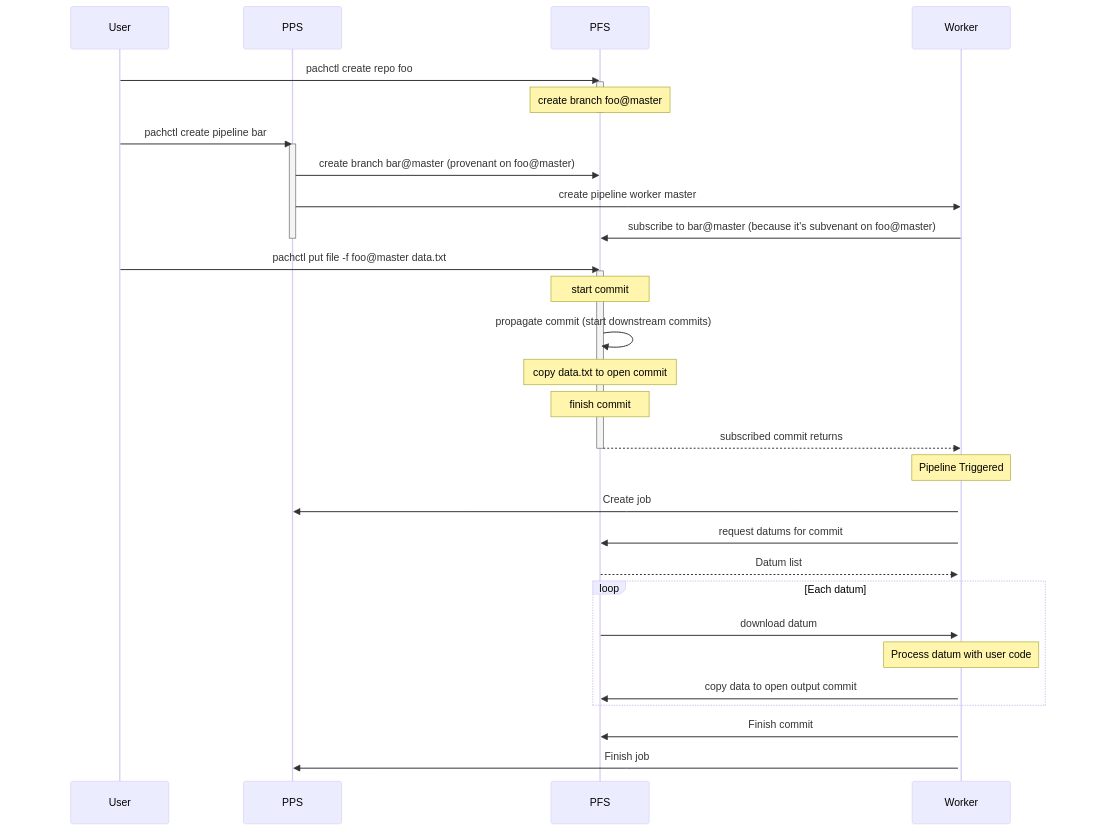
\includegraphics[width=17cm]{graphics/pipeline_communication_sld.png}
  \caption[Swimlane Diagram of the communication between the user and Pachyderm]{Swimlane Diagram of the communication between the user and Pachyderm}
  \label{abb:pipeline_communication_sld}
\end{figure}
\footnotetext{Taken from: \cite{IntroPipelines2023}}



%% ================================ Code =======================================


\anhang{Minikube installation instructions}
\label{appendix:minikube_installation_instructions}
\lstinputlisting{../quellen/minikube_installation_instructions.md}

\newpage
\anhang{Kubernetes setup scripts}

\anhangteil{Ansible setup script}
\label{appendix:ansible_setup_script}
\lstinputlisting{../../Project/Kubernetes_Setup/kluster/setup_scripts/join_cluster.yaml}

\newpage
\anhangteil{Flannel configuration}
\label{appendix:flannel_config}
\lstinputlisting{../../Project/Kubernetes_Setup/kube-flannel.yml}

% \anhangteil{Bash setup script}
% \label{appendix:bash_setup_script}
% \lstinputlisting{../../Project/Kubernetes_Setup/kluster/setup_scripts/setup.sh}

\newpage
\anhangteil{Bash verification script}
\label{appendix:bash_verification_script}
\lstinputlisting{../../Project/Kubernetes_Setup/kluster/setup_scripts/double_check.sh}
